% !TeX spellcheck = en_US
\documentclass[french]{yLectureNote}

\title{Séries - Analyse 2}
\subtitle{Chimie}
\author{Paulhenry Saux}
\date{\today}
\yLanguage{Français}

\professor{IHallery}%isabelle.hallery@univ-tlse3.fr
\usepackage{graphicx}%----pour mettre des images
\usepackage[utf8]{inputenc}%---encodage
\usepackage{geometry}%---pour modifier les tailles et mettre a4paper
%\usepackage{awesomebox}%---pour les boites d'exercices, de pbq et de croquis ---d\'esactiv\'e pour les TP de PC
\usepackage{tikz}%---pour deiffner + d\'ependance de chemfig
\usepackage{tkz-tab}
\usepackage{chemfig}%---pour deiffner formules chimiques
\usepackage{chemformula}%---pour les formules chimiques en \'equation : \ch{...}
\usepackage{tabularx}%---pour dimensionner automatiquement les tableaux avec variable X
\usepackage{awesomebox}%---Pour les boites info, danger et autres
\usepackage{menukeys}%---Pour deiffner les touches de Calculatrice
\usepackage{fancyhdr}%---pour les en-t\^ete personnalis\'ees
\usepackage{blindtext}%---pour les liens
\usepackage{hyperref}%---pour les liens (\`a mettre en dernier)
\usepackage{caption}%---pour la francisation de la l\'egende table vers Tableau
\usepackage{pifont}
\usepackage{array}%---pour les tableaux
\usepackage{lipsum}
\usepackage{yFlatTable}
\usepackage{multicol}
\newcommand{\Lim}[1]{\lim\limits_{\substack{#1}}\:}
\renewcommand{\vec}{\overrightarrow}
\newcommand{\N}[0]{\mathbb{N}}
\begin{document}
\setcounter{chapter}{2}
\chapter{Optique }
\section{Lentille convergente}
\subsection{OR-IR}
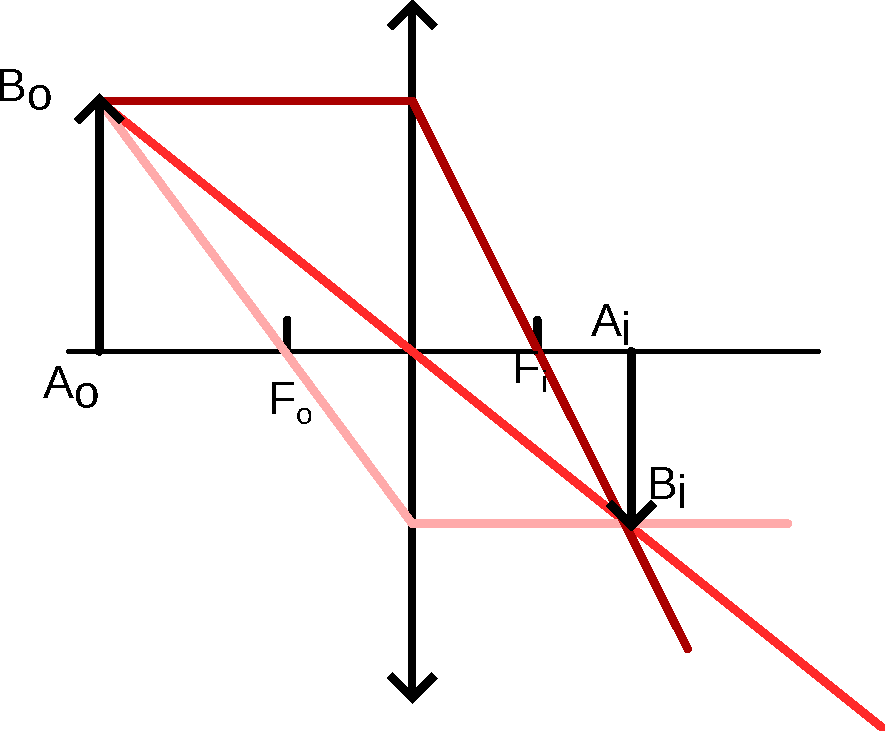
\includegraphics[scale=0.25]{path1}
\checkInfo{Routine de début de TP}{
\begin{enumerate}
 \item Identifier les lentilles convergentes : Celles qui agrandissent lorsque placés à quelques cm de la paillaissae sont convergentes et celles qui rapetissent sont divergente.
 \item Identifier la distance focale avec la méthode d'autocollimation : On colle un miroir sur une lentille et on bouge l'ensemble pour obtenir une image nette sur l'objet.
\end{enumerate}}
\begin{itemize}
 \item Grandissement transversal : On fait simplement le rapport de l'image obtenu sur l'objet
 \item Mesure de \(p_i\) : Il s'agit de la distance entre l'écran et la lentille.
\end{itemize}
\tipsInfo{Incertitude liée à \(p_i\)}{
\(p_i\) est une distance mesurée entre 2 points : la lentille et l'écran. Il y a donc 2 incertitudes à prendre à compte, celle sur la position  de l'écran (\(\frac{1}{\sqrt{3}}\)) et celle liée à l'incertitude de mise au point de l'écran.

Pour l'obtenir, il faut déplacer l'écran après la mesure et avant la mesure pour obtenir l'intervalle dans lequel l'image parait encore nette. On somme ensuite les 2 incertitudes obtenues, bien que la dernière soit normalement plus grande.}
\subsection{OR-IV}
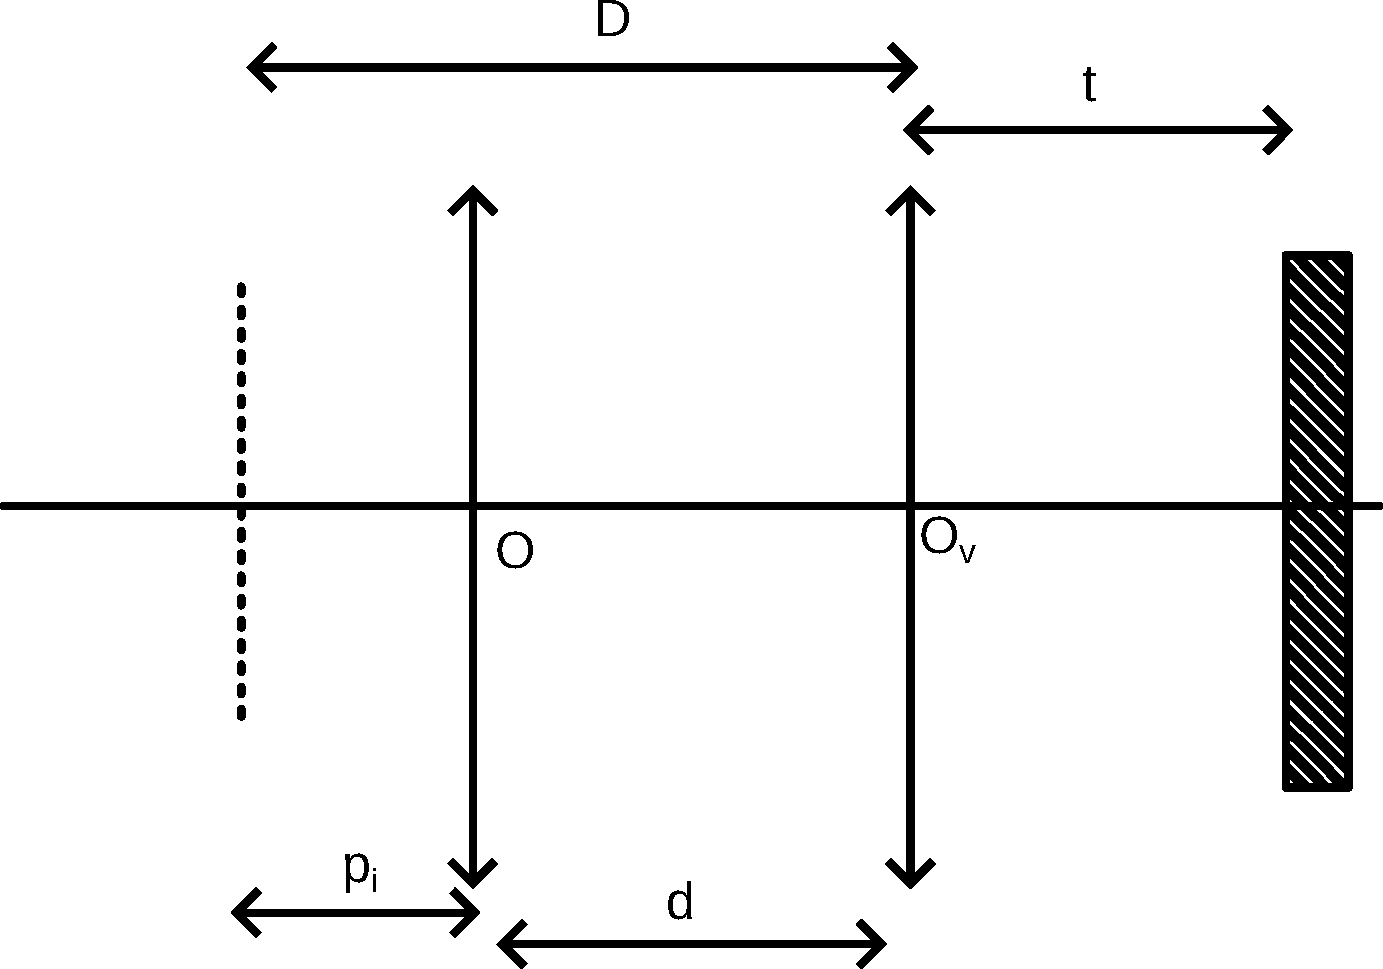
\includegraphics[scale=0.25]{path2}
Ici, on rajoute le viseur pour pouvoir transformer l'image virtuelle obtenue en image réelle que l'on peut observer.
\warningInfo{Viseur}{Il faut penser à régler et mesurer l'incertitude du viseur avant de commencer les mesures avec ce dernier. Pour ce faire, on le place à la distance \(p_{o,v}\) que l'on souhaite et on mesure \(p_{i,v}\) et éventuellement le grandissement.}
\begin{itemize}
 \item Grandissement transversal : On a la relation \(G_{t, r} = \frac{G_{t, o}}{G_{t, v}}\). Lorsque le viseur est en configuration 4f, (i.e. avec un objet à -2f de la lentille et une image à +2f), on a \(G_{t, v} = -1\).
 \item Mesure de \(p_i\) : On mesure expérimentalement la distance entre la lentille étudiée et la lentille du viseur. On a donc la relation : \(p_i = D-d\) avec D la distance frontale et d la distance mesurée expérimentalement.
\end{itemize}
\tipsInfo{Incertitude liée à \(p_i\)}{
\(p_i\) est une  somme de 2 distance, avec chacune leur incertitude :
\begin{itemize}
 \item \(u(D+t) = u(p_{o,v}) + u(p_{i,v}) = \frac{1}{\sqrt{3}} + \) incertitude de mise au point de l'écran.
 \item \(u(d)=\) incertitude de mise au point habituelle.
\end{itemize}
}
\subsection{OV-IR}
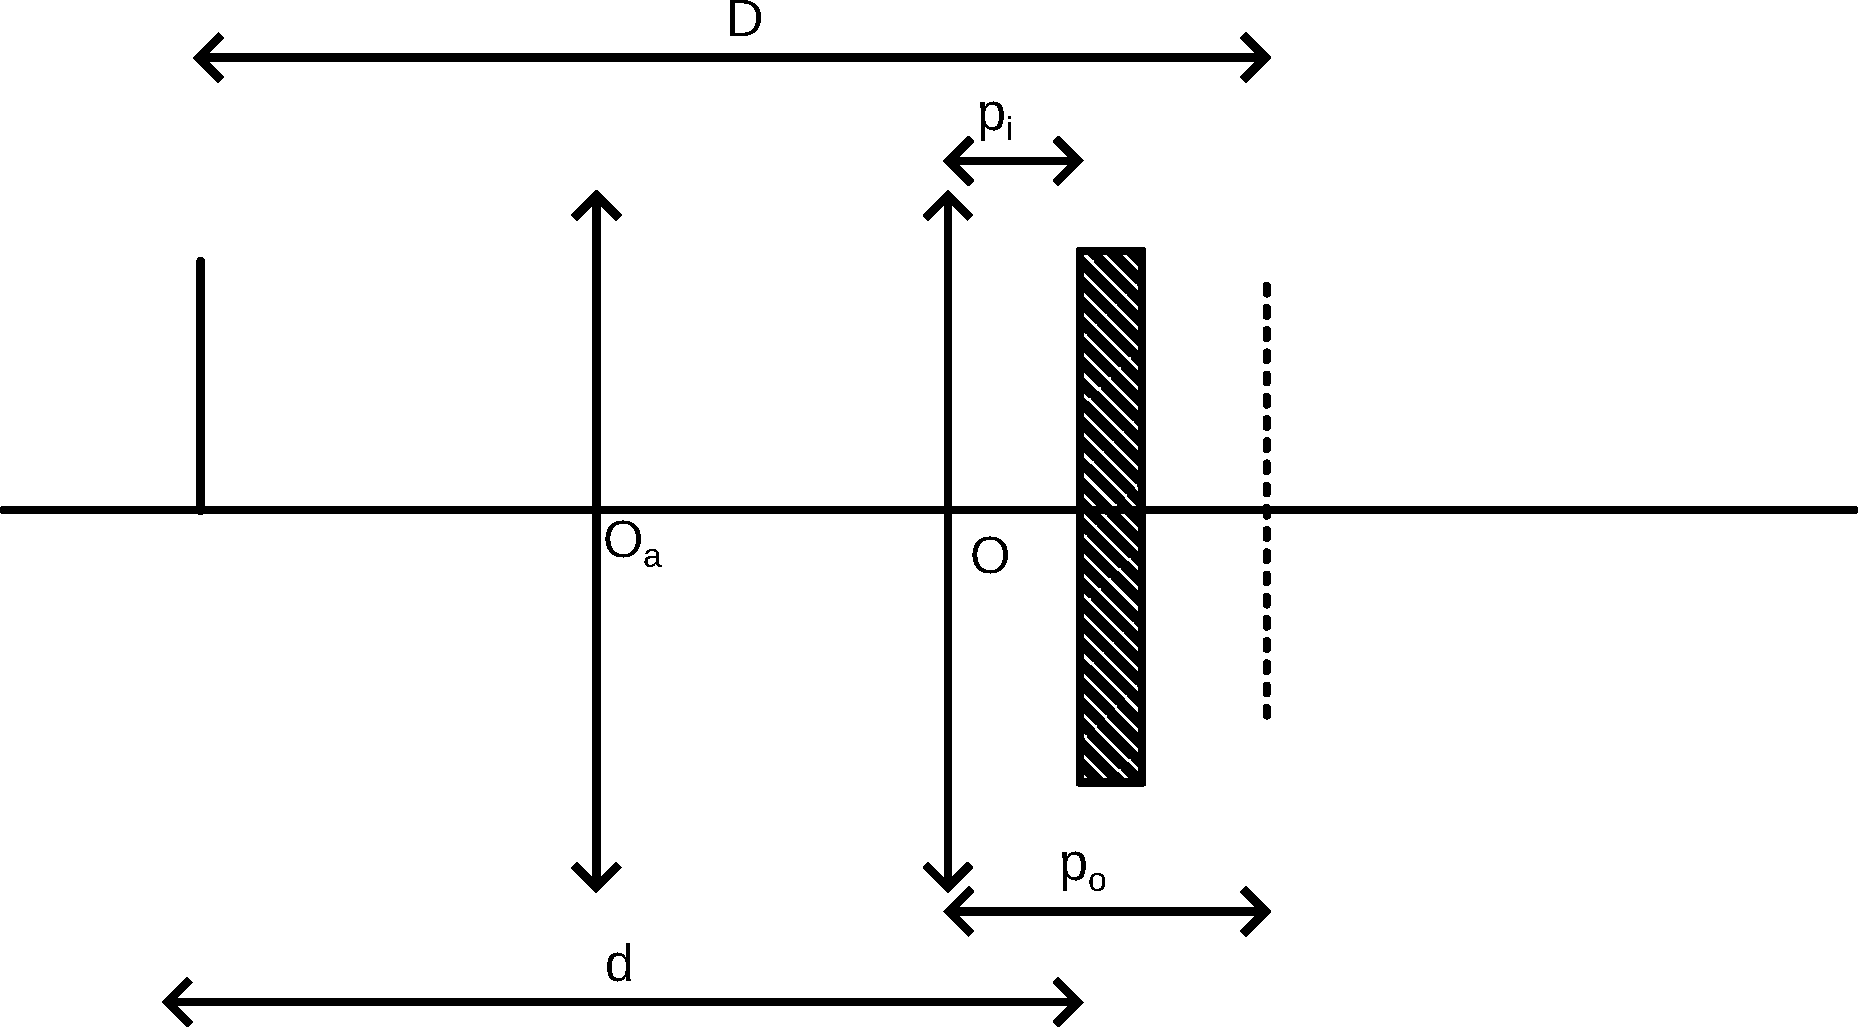
\includegraphics[scale=0.25]{path3}

On va devoir placer l'objet avant la lentille, ce qui n'est pas possible avec un objet réel normal. On va donc utiliser une lentille auxiliaire.

\warningInfo{Lentille auxiliaire}{Il faut penser à régler et mesurer l'incertitude de la lentille auxiliaire avant de commencer les mesures avec cette dernière. Pour ce faire, on le place à la distance \(p_{o,v}\) que l'on souhaite et on mesure \(p_{i,v}\) (qui sera le point à partir duquel on mesurera la distance \(p_o\)). et éventuellement le grandissement.}

\begin{itemize}
 \item Grandissement transversal : On a la relation \(G_{t, r} = \frac{G_{t, o}}{G_{t, aux}}\). Lorsque le viseur est en configuration 4f, (i.e. avec un objet à -2f de la lentille et une image à +2f), on a \(G_{t, v} = -1\).
 \item Mesure de \(p_i\) : On mesure expérimentalement la distance entre l'objet réel de la première lentille et l'écran.
\end{itemize}

\tipsInfo{Incertitude liée à \(p_i\)}{
S'agissant d'une image réelle, c'est la meme que dans le premier cas.
}
\tipsInfo{Incertitude liée à \(p_o\)}{
Il s'agit de l'incertitude d'une mesure pour une lentille convergente de \(p_i\) avec la combinaison OR-IR
}
\criticalInfo{Mesure quand \(p_o = 0\)}{
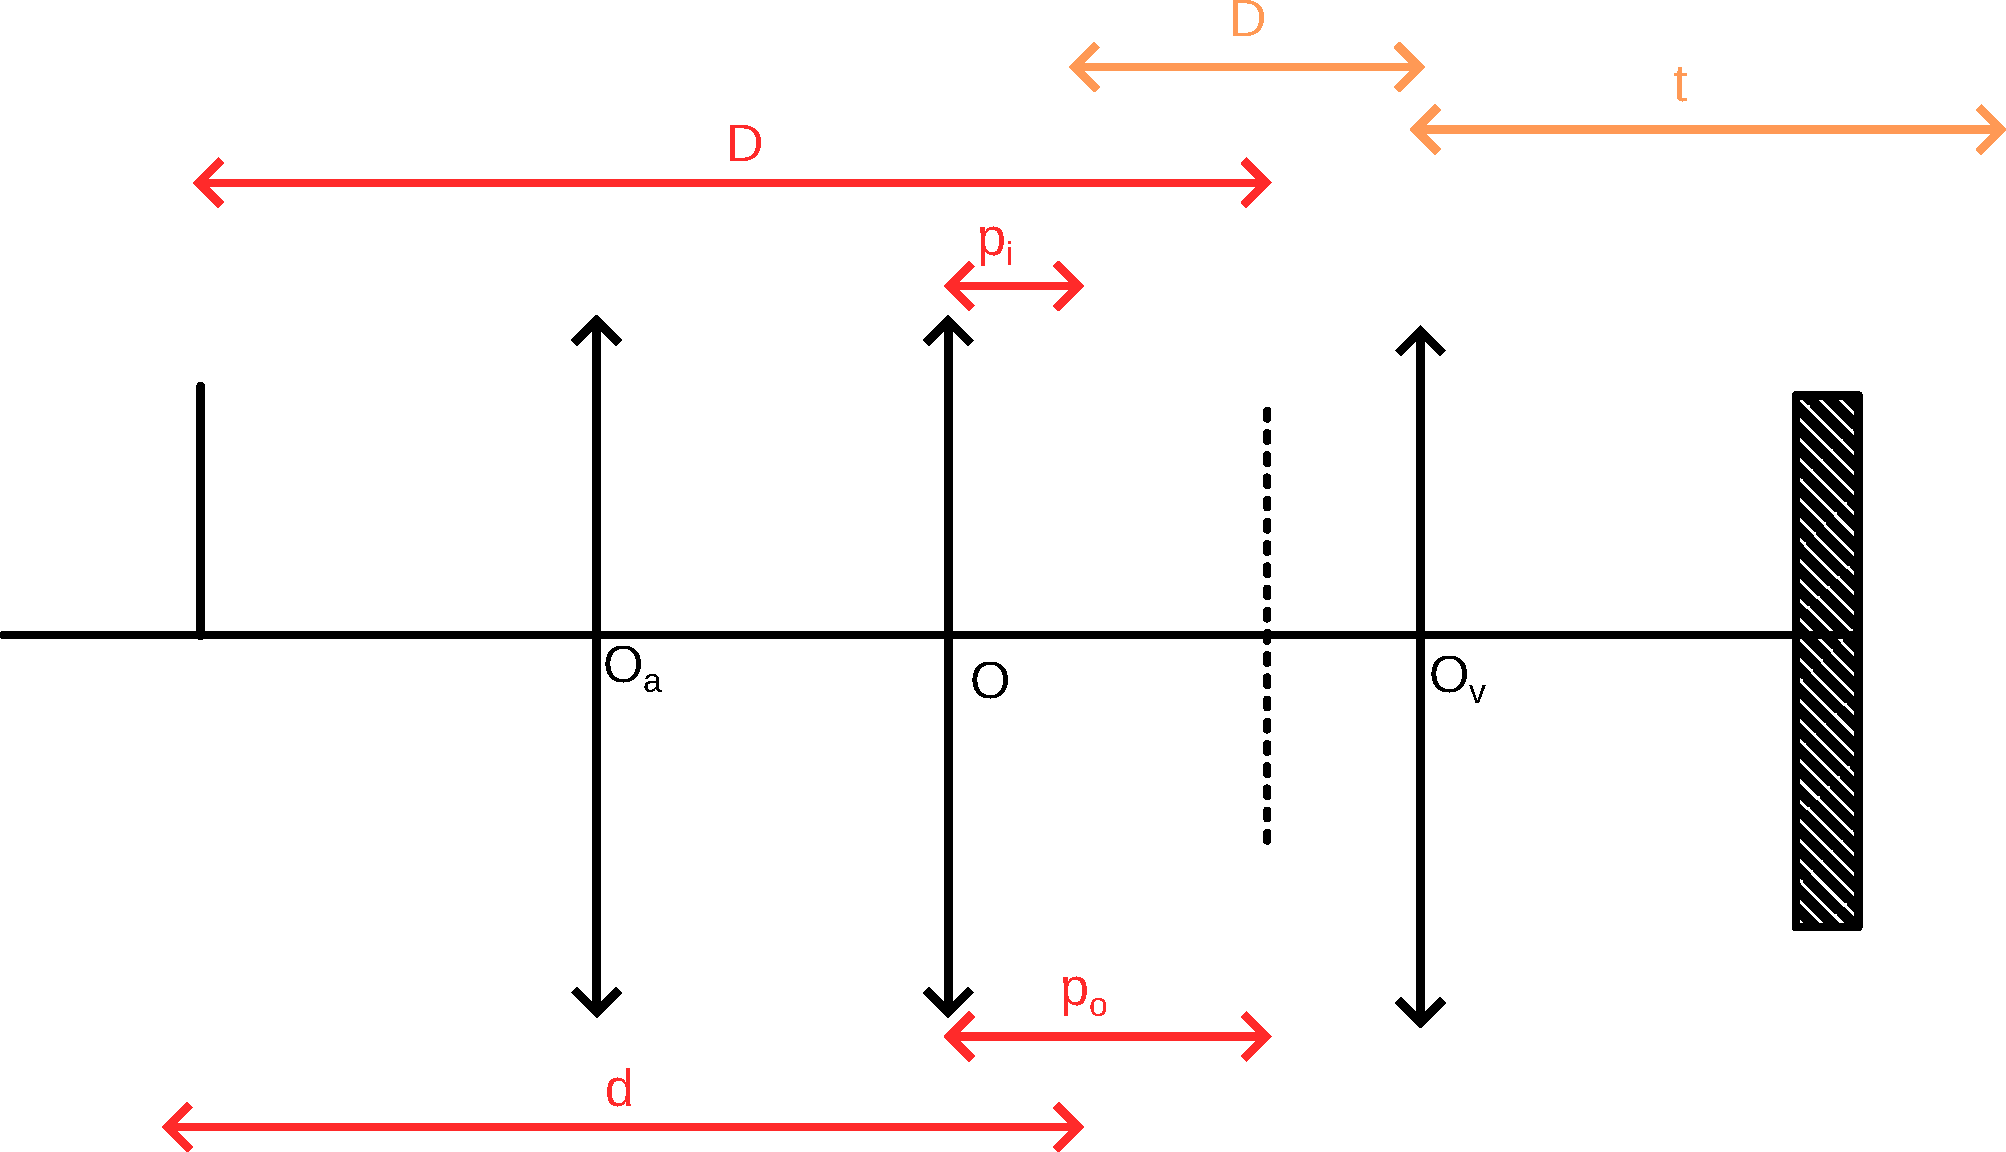
\includegraphics[scale=0.25]{path4}

Quand \(p_o=0\), la distance recherché est de l'ordre du centimètre et on ne peut pas placer l'écran sufisamment proche de la lentille pour obtenir une image nette. Il faut donc utiliser le viseur pour mesurer précisément l'image.

On a alors la relation \(p_i = {\color{orange}d-D}\) et l'incertitude est la somme de l'incertitude de position de la lentille, l'incertitude de mise au point du viseur et l'incertitude de mise au point de la mesure.}
\section{Lentille divergente}
On applique les m\^emes méthodes pour la mesure des OR-IV et OV-IR.
\subsection{OV-IV}
Nous allons combiner ici les méthodes des des OR-IV et OV-IR en utilisant un viseur pour observer l'image et une lentille auxiliaire pour créer l'image virtuelle. Nous serons donc dans la situation suivante :

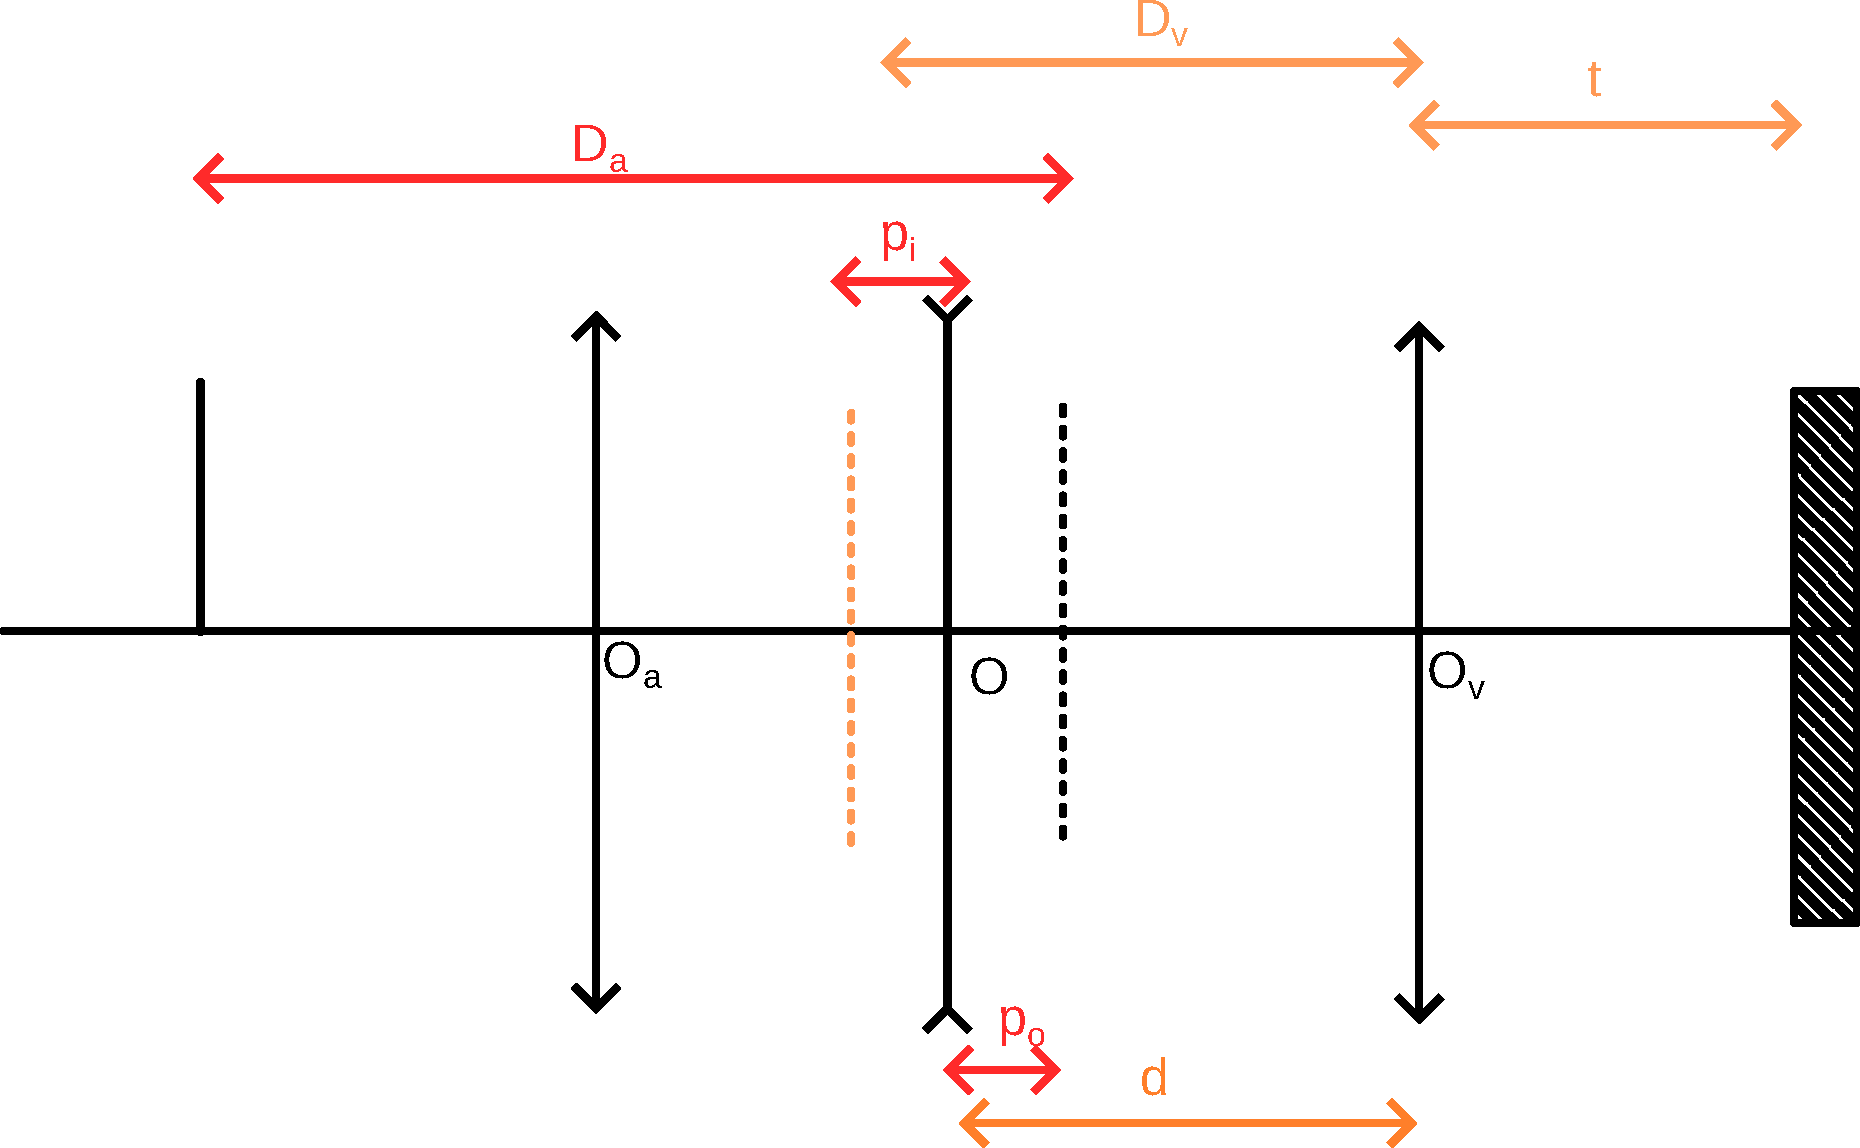
\includegraphics[scale=0.25]{path5}

On peut aussi modéliser par \[A_{o, aux} \xrightarrow{L_{aux}} A_{i, aux} = A_{O}\xrightarrow{L} A_{i} = A_{o, vis}\xrightarrow{L_{vis}} A_{i,vis}\]
\begin{itemize}
 \item Grandissement transversal : On a la relation \(G_{t, r} = \frac{G_{t, o}}{G_{t, aux}\cdot G_{t, vis}}\). Lorsque le viseur et la lentille auxiliare sont en configuration 4f, (i.e. avec un objet à -2f de la lentille et une image à +2f), on a \(G_{t, r} = G_{t, o}\).
 \item Mesure de \(p_i\) : On mesure expérimentalement la distance entre la lentille étudiée et la lentille du viseur. On a donc la relation : \(p_i = D-d\) avec D la distance frontale et d la distance mesurée expérimentalement.
\end{itemize}
\tipsInfo{Incertitude liée à \(p_i\)}{
\(p_i\) est une  somme de 2 distance, avec chacune leur incertitude :
\begin{itemize}
 \item \(u(D) = u(p_{o,v}) + u(p_{i,v}) = \frac{1}{\sqrt{3}} + \) incertitude de mise au point de l'écran.
 \item \(u(d)=\) incertitude de mise au point habituelle.
\end{itemize}
}

\tipsInfo{Incertitude liée à \(p_o\)}{
Il s'agit de l'incertitude d'une mesure pour une lentille convergente de \(p_i\) avec la combinaison OR-IR
}
\section{Modélisation}
\subsection{résultats théoriques}
On peut vérifier que les résultats sont cohérents avec
\begin{theorem}[Valeur de \(p_i\)]
\[\bar{P_i}   = \frac{1}{V+\frac{1}{\bar{p_o}}}\]
\end{theorem}
\begin{theorem}[Valeur de grandissement]
\[G_t = \frac{\bar{p_i}}{\bar{p_o}}\]
\end{theorem}
\subsection{Détermination de la vergence}
À partir de la relation de Descartes et de celle du grandissement, on obtient les relations suivantes

\begin{theorem}
  \[G_t = -V\bar{p_i}+1\]
  \[Gt^{-1} = \bar{p_o}V+1\]
  \[\bar{p_i}^{-1} = \bar{p_o}^{-1}+V\]
\end{theorem}
\section{Résumé des incertitudes}
\checkInfo{Mesure une incertitude de mise au point}{On prend le milieu de l'intervalle comme valeur et on divise par 2 pour l'incertitude}
\criticalInfo{Montage 4f}{On prend quand c'est possible un montage de type 4f quand c'est possible pour réduire l'incertitude.}
\subsection{Objet réel}
\begin{itemize}
 \item Incertitude de position liée à l'incertitude de lecture sur la règle graduée de la lentille
 \item Incertitude de position liée à l'incertitude de lecture sur la règle graduée de l'écran
\end{itemize}
\subsection{Objet virtuel}
\begin{itemize}
 \item Incertitude de position liée à l'incertitude de lecture sur la règle graduée de la lentille étudiée
 \item Incertitude de mise au point de la lentille auxiliaire utilisée
\end{itemize}
\subsection{Image réelle}
\begin{itemize}
 \item Incertitude de position liée à l'incertitude de lecture sur la règle graduée de la lentille
 \item Incertitude de mise au point de l'écran
\end{itemize}
\subsection{Image virtuelle}
\begin{itemize}
 \item Incertitude de position liée à l'incertitude de lecture sur la règle graduée de la lentille étudiée
 \item Incertitude de mise au point du viseur
 \item Incertitude de mise au point du viseur à tirage fixée
\end{itemize}
\end{document}

